\chapter{LIGHT FIELD IMAGE}
Light Field (campo luminoso) si riferisce alla quantità di luce in funzione della posizione e della direzione, ovvero una funzione vettoriale 4D nello spazio libero. Il campo luminoso  è stato introdotto nella computer graphics nel 1996 da Levoy e Hanrahan, i quali hanno proposto un sistema di rendering basato su immagini (IBR) e sul campo luminoso registrato di una scena. Tale sistema IBR è potente nel rendering di nuove view, non solo con il cambiamento del punto di vista, ma anche per il punto focale cambiato, noto come ri-messa a fuoco. Tuttavia, la registrazione del campo luminoso 4D non è banale poiché i sensori di immagini esistenti sono progettati per l'imaging 2D. Una fotocamera tradizionale cattura solo una rappresentazione piatta e bidimensionale dei raggi di luce che raggiungono l’obiettivo in una data posizione. Il sensore di immagine 2D registra la somma della luminosità e del colore di tutti i raggi luminosi che arrivano a ogni singolo pixel. Al contrario, una light field camera può registrare non solo i valori di luminosità e colore nel sensore di immagini 2D, ma anche la direzione/l’angolo di tutti i raggi luminosi che arrivano al sensore. Queste informazioni aggiuntive ci permettono di ricostruire da dove proveniva esattamente ogni raggio di luce prima di raggiungere la telecamera, rendendo possibile il calcolo di un modello tridimensionale della scena catturata. 
\begin{figure}[ht]
    \centering
    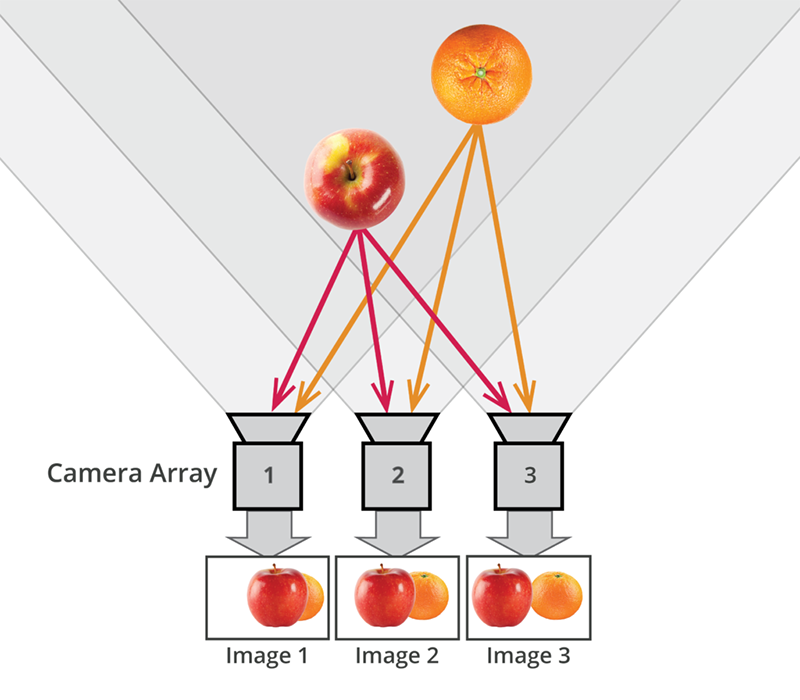
\includegraphics{img/what-is-a-light-field-disparity-recording-lytro.png}
    \caption{Cattura di un ligth field}
    \label{fig:ligthFieldRecording}
\end{figure}
\\
\\
I light field possono essere catturati utilizzando diverse tecniche, tra cui:
\begin{itemize}
    \item una singola telecamera controllata roboticamente,
    \item un arco rotante di telecamere,
    \item una serie di telecamere o moduli telecamere,
    \item una singola fotocamera dotata di un array di microlenti.
\end{itemize}

A seconda della tecnica utilizzata, i dati dell'immagine acquisita sono tipicamente costituiti da un’immagine contenente molte immagini secondarie (ottenute da un singolo sensore e una matrice di microlenti) o molte immagini (da più fotocamere o esposizioni). 
Entrambi i set di dati mostrano immagini con leggere variazioni, poiché catturano raggi di luce da diverse angolazioni nello spazio. Queste variazioni permettono di determinare la posizione degli oggetti e di creare un volume di campo luminoso 3D. Tuttavia, le fotocamere plenottiche come Lytro e Raytrix, sebbene offrano nuove opportunità, richiedono una compressione efficace per gestire le dimensioni considerevoli delle immagini raw e la loro rappresentazione non convenzionale, mantenendo al contempo la qualità dell'immagine.
\begin{figure}[ht!]
    \centering
    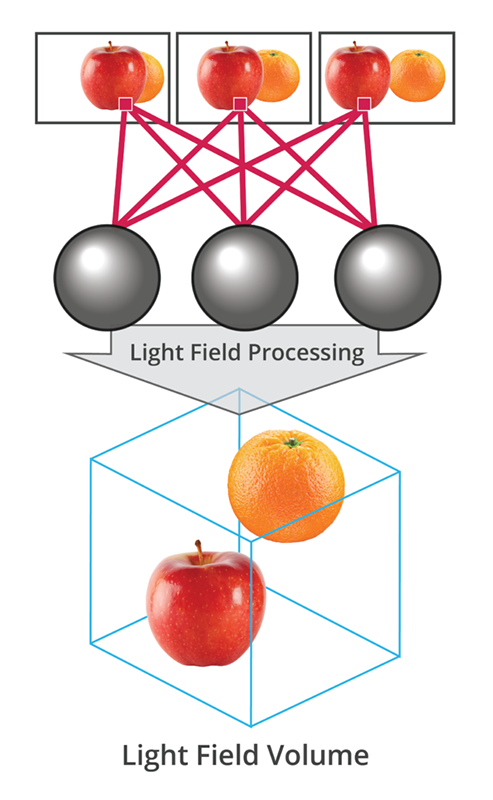
\includegraphics{img/what-is-a-light-field-disparity-processing-lytro.png}
    \caption{Informasioni racchiuse in un ligth field}
    \label{fig:ligthFieldInfo}
\end{figure}